\documentclass[final]{beamer}
%% Possible paper sizes: a0, a0b, a1, a2, a3, a4.
%% Possible orientations: portrait, landscape
%% Font sizes can be changed using the scale option.
\usepackage[size=a1,orientation=portrait,scale=1.1]{beamerposter}
\usetheme{gemini}
\usecolortheme{seagull}
\useinnertheme{rectangles} 
% ====================
% Packages
% ====================
\usepackage[utf8]{inputenc}
\usepackage{graphicx}
\usepackage{booktabs}
\usepackage{tikz}
\usepackage{pgfplots}
\usepackage{svg}
\usepackage{amsmath,amssymb,amsfonts}
\usepackage{multicol}
\usepackage{placeins}
\usepackage[noend]{algpseudocode}
\usepackage{amsmath}
% ====================
% Lengths
% ====================
% If you have N columns, choose \sepwidth and \colwidth such that
% (N+1)*\sepwidth + N*\colwidth = \paperwidth
\newlength{\sepwidth}
\newlength{\colwidth}
\setlength{\sepwidth}{0.03\paperwidth}
\setlength{\colwidth}{0.45\paperwidth}
\newcommand{\separatorcolumn}{\begin{column}{\sepwidth}\end{column}}
% ====================
% Logo (optional)
% ====================
% LaTeX logo taken from https://commons.wikimedia.org/wiki/File:LaTeX_logo.svg
% use this to include logos on the left and/or right side of the header:
\logoleft{
\includegraphics[height=6.6cm]{logo/CSE.png}}
\logoright{
\includegraphics[height=6.6cm]{logo/iub.png}}
% ====================
% Footer (optional)
% ====================
\footercontent{
	\insertdate \hfill
	Algorithm Project \hfill
	CSE211: Algorithms Lab
    % \href{mailto:myemail@exampl.com}{\texttt{myemail@example.com}}
    }
% (can be left out to remove footer)
% ====================
% My own customization
% - BibLaTeX
% - Boxes with tcolorbox
% - User-defined commands
% ====================
% ====================
% BibLaTeX
% ====================

\usepackage[backend=biber,
	bibstyle=authoryear,
	citestyle=authoryear,
	style=authoryear,
	maxcitenames=2,
	maxbibnames=20, % limit the length of list of names (authors/editors/etc.)
	sorting=ydnt, % sort references by year (descending), name, title
	dashed=false, % show authors instead of dash in publications having the same authors
	giveninits=true % render authors' given name initials and not the full given names
]{biblatex}
%% Biblatex with Beamer bibliography icons
\setbeamertemplate{bibliography item}{%
	\ifboolexpr{ test {\ifentrytype{book}} or test {\ifentrytype{mvbook}}
		or test {\ifentrytype{collection}} or test {\ifentrytype{mvcollection}}
		or test {\ifentrytype{reference}} or test {\ifentrytype{mvreference}} }
	{\setbeamertemplate{bibliography item}[book]}
	{\ifentrytype{online}
		{\setbeamertemplate{bibliography item}[online]}
		{\setbeamertemplate{bibliography item}[article]}}%
	\usebeamertemplate{bibliography item}}
\defbibenvironment{bibliography}
{\list{}
	{\settowidth{\labelwidth}{\usebeamertemplate{bibliography item}}%
		\setlength{\leftmargin}{\labelwidth}%
		\setlength{\labelsep}{\biblabelsep}%
		\addtolength{\leftmargin}{\labelsep}%
		\setlength{\itemsep}{\bibitemsep}%
		\setlength{\parsep}{\bibparsep}}}
{\endlist}
{\item}
%% Redefine \refname
\renewcommand{\bibname}{References}
%% Redefine \parencite to use square brackets instead of braces
\DeclareCiteCommand{\parencite}
{\usebibmacro{prenote}}
{\usebibmacro{citeindex}%
	\printtext[bibhyperref]{[\usebibmacro{cite}]}}
{\multicitedelim}
{\usebibmacro{postnote}}
%% Highlight author names using Beamer data annotation
%% Usage: add a new line `author+an = {<author-order>=highlight}` to an entry
%% For example: author+an = {3=highlight} => highlight the 3rd author name
\AtBeginBibliography{
	\renewcommand*{\mkbibnamegiven}[1]{%
		\ifitemannotation{highlight}
		{\textbf{#1}}
		{#1}%
	}
	
	\renewcommand*{\mkbibnamefamily}[1]{%
		\ifitemannotation{highlight}
		{\textbf{#1}}
		{#1}%
	}
}

% ====================
% Boxes with tcolorbox
% ====================
\usepackage[most]{tcolorbox}

%%% Beamer colors in boxes

\newcommand{\beamercolorsinboxes}[1]{
	\setbeamercolor{itemize item}{fg=#1!75!black}
	\setbeamercolor{itemize/enumerate body}{fg=#1!65!white}
	\setbeamercolor{itemize/enumerate subbody}{fg=#1!65!white}
	\setbeamercolor{item projected}{fg=white, bg=#1!75!black}
}

%%% Highlight Oval Box
\newtcbox{\xmybox}[1][red]{on line,
	arc=7pt,colback=#1!10!white,colframe=#1!50!black,
	before upper={\rule[-3pt]{0pt}{10pt}},boxrule=1pt,
	boxsep=0pt,left=6pt,right=6pt,top=2pt,bottom=2pt}
%%% Box for stating problems
%%%%%%%%
%Usage: (similar for infobox)
%	\begin{defbox}{title}
	%		contents
	%	\end{defbox}
%%%%%%%%
\newtcolorbox{defbox}[1]{%
	enhanced,
	attach boxed title to top 	left={xshift=5mm,yshift=-5mm,yshifttext=-5mm},
	colback=cyan!5!white,
	colframe=cyan!75!black,
	coltitle=cyan!80!black,
%	left=0mm,right=0mm,top=2mm,bottom=0mm,
	title={#1},
	fonttitle=\bfseries\large, fontupper=\color{cyan!65!white},
	boxed title style={colback=cyan!5!white,colframe=cyan!75!black},
	before upper={
		\beamercolorsinboxes{cyan}
	}
}%
%%% Box for announcement
\newtcolorbox{infobox}[1]{%
	enhanced,
	attach boxed title to top 	left={xshift=5mm,yshift=-5mm,yshifttext=-5mm},
	colback=yellow,
	colframe=red!75!black,
	coltitle=red!75!black,
%	left=0mm,right=0mm,top=2mm,bottom=0mm,
	title={#1},
	fonttitle=\bfseries\large, fontupper=\color{red!65!white},
	boxed title style={colback=yellow,colframe=red!75!black},
	before upper={
		\beamercolorsinboxes{red}
	}
}%
%%% Box for example
\newtcolorbox{exabox}[1]{%
	enhanced,
	attach boxed title to top 	left={xshift=5mm,yshift=-5mm,yshifttext=-5mm},
	colframe=brown!75!black,colback=brown!5!white,coltitle=brown!50!brown!75!black,
%	left=0mm,right=0mm,top=2mm,bottom=0mm,
	title={#1},
	fonttitle=\bfseries\large, fontupper=\color{brown!65!white},
	boxed title style={colback=brown!5!white,coltitle=brown!50!brown!75!black},
	before upper={
		\beamercolorsinboxes{brown}
	}
}%
%%% Theorem Box
%%%%%%%%
%Usage: (similar for conjecture, lemma, etc.)
%	\begin{thm}{title}{nameref}
	%		contents
	%	\end{thm}
% Use \ref{thm:nameref} to refer to the theorem
%%%%%%%%
%%%% Use \newtcbtheorem[number within=section]{thm} to number within each section
\newtcbtheorem[]{thm}%
{Theorem}{attach boxed title to top 	left={xshift=5mm,yshift=-5mm,yshifttext=-5mm},
	enhanced jigsaw,
	%	top=2mm,bottom=0mm,left=0mm,right=0mm,
	fonttitle=\bfseries\large,fontupper=\itshape\color{blue!65!white},
	colframe=blue!75!black,colback=blue!5!white,coltitle=blue!50!blue!75!black,
	boxed title style={colback=blue!5!white,coltitle=blue!50!blue!75!black},
	before upper={
		\beamercolorsinboxes{blue}
	}
}{thm}%
%%% Proposition Box
\newtcbtheorem[use counter from=thm]{prop}%
{Proposition}{attach boxed title to top 	left={xshift=5mm,yshift=-5mm,yshifttext=-5mm},
	enhanced jigsaw,
	%	top=2mm,bottom=0mm,left=0mm,right=0mm,
	fonttitle=\bfseries\large,fontupper=\itshape,
	colframe=gray!75!black,colback=gray!5!white,coltitle=gray!50!gray!75!black,
	boxed title style={colback=gray!5!white,coltitle=gray!50!gray!75!black},
	before upper={
		\beamercolorsinboxes{gray}
	}
}{prop}%
%%% Conjecture Box
\newtcbtheorem[use counter from=thm]{conj}%
{Conjecture}{attach boxed title to top 	left={xshift=5mm,yshift=-5mm,yshifttext=-5mm},
	enhanced jigsaw,
	%	top=2mm,bottom=0mm,left=0mm,right=0mm,
	fonttitle=\bfseries\large,fontupper=\slshape,
	colframe=orange!75!black,colback=orange!5!white,coltitle=orange!50!orange!75!black,
	boxed title style={colback=orange!5!white,coltitle=orange!50!orange!75!black},
	before upper={
		\beamercolorsinboxes{orange}
	}
}{conj}%
%%% Lemma Box
\newtcbtheorem[use counter from=thm]{lem}%
{Lemma}{attach boxed title to top 	left={xshift=5mm,yshift=-5mm,yshifttext=-5mm},
	enhanced jigsaw,
	%	top=2mm,bottom=0mm,left=0mm,right=0mm,
	fonttitle=\bfseries\large,fontupper=\itshape,
	colframe=green!75!black,colback=green!5!white,coltitle=green!50!green!75!black,
	boxed title style={colback=green!5!white,coltitle=green!50!green!75!black},
	before upper={
		\beamercolorsinboxes{green}
	}
}{lem}%
%%% Claim Box
\newtcbtheorem[use counter from=thm]{clm}%
{Claim}{attach boxed title to top 	left={xshift=5mm,yshift=-5mm,yshifttext=-5mm},
	enhanced jigsaw,
	%	top=2mm,bottom=0mm,left=0mm,right=0mm,
	fonttitle=\bfseries\large,fontupper=\itshape,
	colframe=pink!75!black,colback=pink!5!white,coltitle=pink!50!pink!75!black,
	boxed title style={colback=pink!5!white,coltitle=pink!50!pink!75!black},
	before upper={
		\beamercolorsinboxes{pink}
	}
}{clm}%
%Configs
\def\inst#1{\unskip$^{#1}$}
\def\orcidID#1{\unskip$^{[#1]}$} % added MR 2018-03-10
\def\fnmsep{\unskip$^,$}
\def\email#1{{\tt#1}}
\renewcommand{\pgfuseimage}[1]{\includegraphics[scale=2.0]{#1}}
\pgfplotsset{compat=1.18}
\title{Merge$&$Search: A Smart Disaster Response System}
\author
{
    Abdullah Mohammad Sadman \inst{1} \and
    Fahim Shahriar \inst{2} \and
    Arman Uddin \inst{3} \and 
    MD Alvee Sarker \inst{4} \and 
    Abdullah Al Hossain\inst{5} \and
    Tanjil Sarker\inst{6}
}
% \institute[shortinst]{\inst{1} Independent University Bangladesh \samelineand \inst{2} Another Institute}
\institute{Department of Computer Science and Engineering\\Independent University, Bangladesh\\Dhaka, Bangladesh.\\
\email{\{2330322$^{1}$,2310688$^{2}$,2311300$^{3}$,2311249$^{4}$,2310778^{5},2312026$^{6}$\}@iub.edu.bd}
%\url{http://www.springer.com/gp/computer-science/lncs} 
}
\date{Autumn, 2024}
\begin{document}
    \begin{frame}[t]
    	\begin{columns}[t]
        	\begin{column}{2\colwidth+\sepwidth}
                \begin{exampleblock}{ A  Dive into Merge Sort and Binary Search Trees}
                	\justifying{
                    Merge Sort and Binary Search Tree  are both \textbf{Divide-and-conquer algorithm with a Dynamic Structure that guarantees stable sorting and searching }each playing a crucial role in efficient data processing and management. Efficient data processing and management are pivotal in various domains, from disaster response to database optimization. Merge Sort and Binary Search Tree
                    stand out as foundational tools for achieving these objectives.  Merge Sort is an efficient, stable sorting algorithm that divides data into smaller subsets, sorts them, and merges the results. A Binary Search Tree (BST) stores data in a hierarchical structure, allowing fast searching, insertion, and deletion. Combining Merge Sort and BST enhances both sorting and searching, providing an effective solution for data organization and efficient querying in real-world applications.  
                    }
            	\end{exampleblock}
        	\end{column}
    	\end{columns}
    	\begin{columns}[t]
    		\separatorcolumn
    		\begin{column}{\colwidth}
    			\begin{block}{Origin and Background}
        			\justifying
                    \textbf{Merge sort}, developed by \textbf{John von Neumann in 1945}, is a divide-and-conquer algorithm that efficiently sorts data. It was introduced in his paper \textbf{"Algorithms for Solving Mathematical Problems."} The method splits arrays into smaller subarrays, sorts them, and merges them back together, making it particularly effective for large datasets and linked lists. \vspace{1em}
                    
                    \textbf{Binary search}, an efficient algorithm for finding an item in a sorted list, dates back to ancient times. Its origins can be traced to the works of mathematicians like \textbf{Euclid and later formalized by John von Neumann in the mid-20th century}. The method halves the search space with each step, making it significantly faster than linear search, especially for large datasets.

    			\end{block}
                \begin{block}{How Both Algorithms are used in Disaster Management}
                    \justifying
                    \textbf{Merge Sort and Binary Search Trees}  are useful in \textbf{disaster management} for efficiently handling large datasets. They help in sorting resources, managing real-time data, and making quick decisions during critical situations.
                    \phantom{This text will be invisible}\\
                    \phantom{This text will be invisible}\\
                    \textbf{\textbf{$Merge Sort$} helps by sorting resources, rescue operations, and GIS data, ensuring quick allocation and decision-making.}
                    \phantom{This text will be invisible}\\
                     \phantom{This text will be invisible}\\
                    \textbf{$BST$ allows efficient storage and retrieval of real-time data like affected areas, rescue teams, and available resources, speeding up searches and updates for better coordination.}
                    \phantom{This text will be invisible}\\
                
                   

                \end{block}
    			\begin{block}{Breakdown}
                    \justifying
                    \textbf{Merge Sort:}
\begin{itemize}
    \item Splits the dataset into smaller parts.
    \item Sorts each part and then merges them into a final ordered dataset.
    \item Helps prioritize and allocate resources (e.g., medical supplies, food) quickly in disaster situations.
\end{itemize}

\textbf{Binary Search Tree (BST):}
\begin{itemize}
    \item Data is stored in a hierarchical structure where each node has a left and right child.
    \item Allows efficient search, insertion, and deletion of real-time data (e.g., locations of affected areas, available rescue teams).
    \item Enhances coordination by providing faster access to critical information during a disaster response.
\end{itemize}

                    
                \end{block}
                \begin{block}{Python Implementation}
                    Here's a python program showcasing the implementation of Merge and BST in Disaster Management\\
                    \phantom{This text will be invisible}\\
                    \centerline{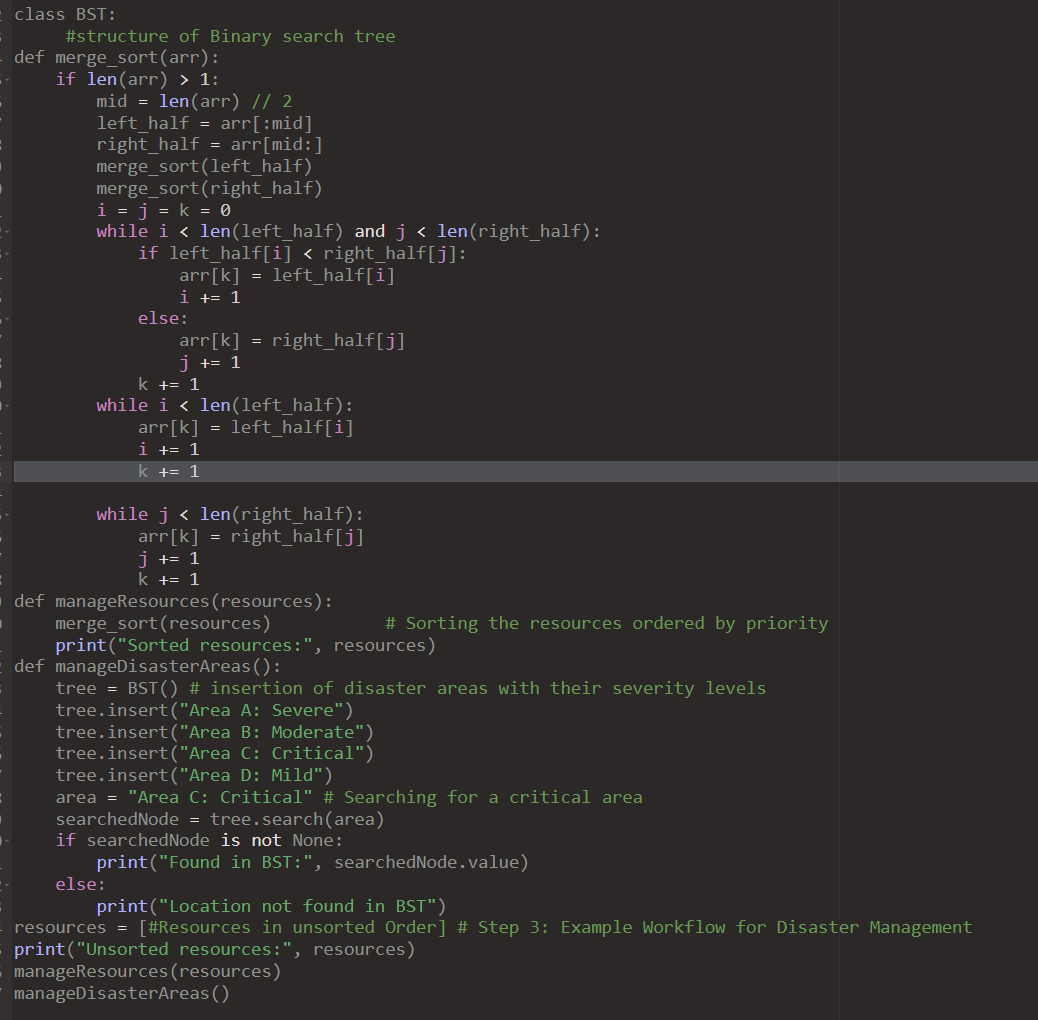
\includegraphics[width=.96\linewidth]{apply}}
                    \phantom{This text will be invisible}\\
                    
                \end{block}
    		\end{column}
    		\separatorcolumn
    		\begin{column}{\colwidth}
    		
       		\begin{block}{Flow Chart}
                \centerline{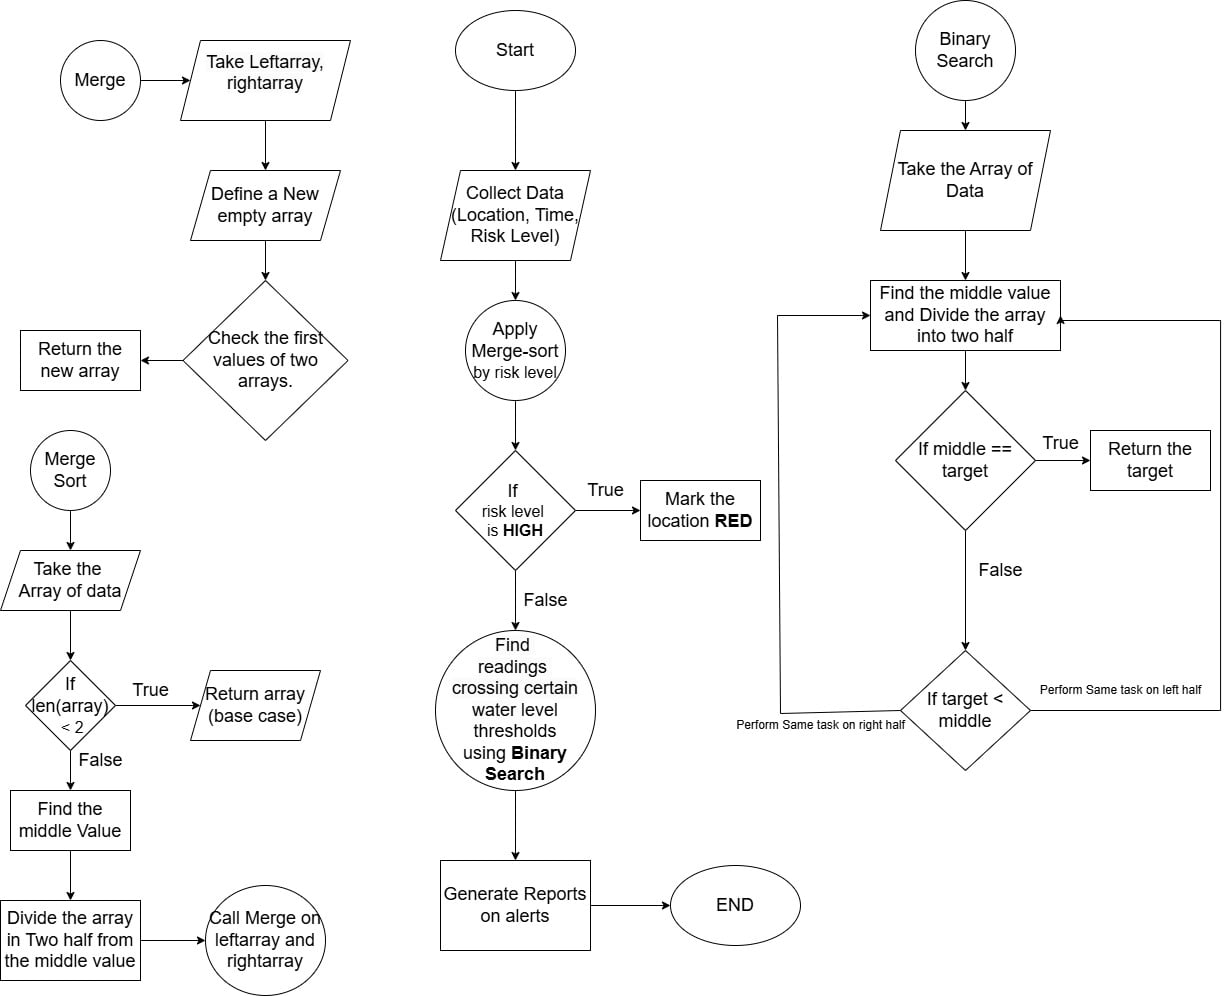
\includegraphics[width=.96\linewidth]{disaster}}
                \centering
                
                \end{block}
                \begin{block}{Complexities Analysis}
                \justifying
                \textbf{Choice of Stable Algorithm:} The implementation combines Merge Sort for sorting resources and Binary Search Tree (BST) operations for inserting and searching disaster areas. Merge Sort provides stable sorting of input elements, while the BST enables efficient organization and lookup of disaster areas.\phantom{This text will be invisible}\\
                \textbf{Divide and Conquer Approach: } Merge Sort follows a divide-and-conquer strategy. The array is repeatedly divided into two equal parts, and sorting occurs as the recursion unwinds. The division takes$O(logn)$  levels, and merging the divided parts takes $O(n)$  time at each level, leading to a total runtime of $O(nlogn)$ \phantom{This text will be invisible}\\
                \textbf{Time Complexity:}$O(nlogn)$
                \textbf{Space Complexity:}$O(n)$

                
                \textbf{Binary Search Tree (BST) Operations: } 
                \phantom{This text will be invisible}\\
                \textbf{  Time Complexity: }$O(h)$ where h is the height of the tree. For a balanced BST,$h  =logn$ giving a time complexity of $O (logn)$
                
                
                
            
\textbf{Overall Efficiency:} Merge Sort and BST operations combine to create an efficient workflow for sorting and managing resources, maintaining the overall time complexity of $O(nlogn)$
                \end{block}
       
                \begin{block}{Real Life Scenario}
                \centerline{\includegraphics[width=.86\linewidth]{h}}
                \justifying 
                \textbf{Flood Forecasting and Warning Centre of Bangladesh }collects and analyzes data(where the given sorting and searching plays vital role) from various sources to predict potential flood events. By issuing timely warnings based on these forecasts, the center helps authorities and communities prepare and respond effectively, minimizing the impact of floods on lives and infrastructure.
     
    		\end{block}
      
                \begin{block}{Conclusion}
        			\justifying
                  In conclusion, the implementation of Merge Sort and Binary Search algorithms in a disaster management system plays a crucial role in ensuring efficient data organization and quick retrieval of critical information during emergency situations. By combining these powerful algorithms, the system can effectively sort and search through data, enabling timely decision-making and response efforts. This innovative approach enhances the system's capability to handle large volumes of data and streamline disaster management processes, ultimately contributing to improved disaster response and mitigation outcomes.
    			\end{block}
               
                
    		\end{column}
    		\separatorcolumn
    	\end{columns}  
    \end{frame}
\end{document}